\section{Design of the Chorus and Flanger Effect}

The flanger and chorus effect are very similar in their design so they will be presented in the same section. \\

From the block diagram presented in section \autoref{chor_flang}, a block diagram in the discrete time domain for the flanger and chorus effect can be obtained and is shown in \autoref{fig:chorus_diag_des}. \\ 
The chorus effect is the one in red and black while the flanger is only in black.  
\begin{figure} [htbp!]
	\centering
\begin{picture}(0,0)%
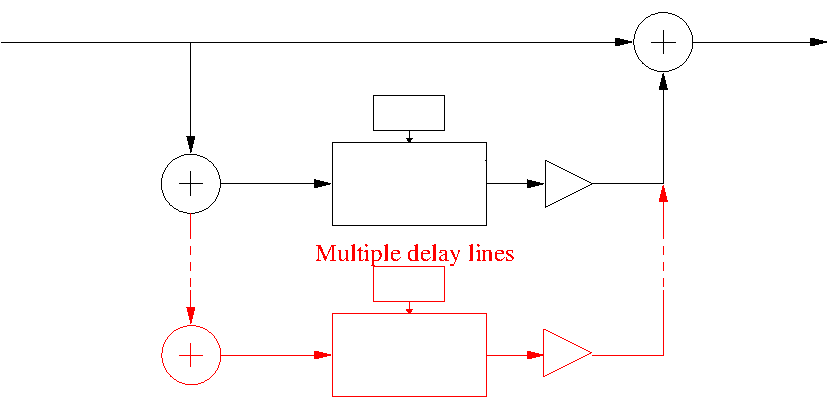
\includegraphics{chorus_diag_des.pdf}%
\end{picture}%
\setlength{\unitlength}{4144sp}%
%
\begingroup\makeatletter\ifx\SetFigFont\undefined%
\gdef\SetFigFont#1#2#3#4#5{%
	\reset@font\fontsize{#1}{#2pt}%
	\fontfamily{#3}\fontseries{#4}\fontshape{#5}%
	\selectfont}%
\fi\endgroup%
\begin{picture}(6327,3018)(3766,-3493)
\put(6571,-1906){\color[rgb]{0,0,0}$z^{-d_{1}}$}%

\put(8101,-1636){\color[rgb]{0,0,0}$g_{1}$}%

\put(6616,-3211){\color[rgb]{1,0,0}$z^{-d_{2}}$}%

\put(8101,-2986){\color[rgb]{1,0,0}$g_{2}$}%

\put(6706,-2671){\color[rgb]{1,0,0}\textit{LFO}}%

\put(6706,-1366){\color[rgb]{0,0,0}\textit{LFO}}%

\put(3781,-646){\color[rgb]{0,0,0}\textit{x[n]}}%

\put(9406,-646){\color[rgb]{0,0,0}\textit{y[n]}}%

\end{picture}%
\caption{Block Diagram of the chorus and flanger effect in the discrete time domain.}
\label{fig:chorus_diag_des}
\end{figure}

From \autoref{fig:chorus_diag_des}, the following differential equations can be inferred:

The equation for the flanger can be written as:
\begin{equation}
\label{flang_eq}
		y[n] = x[n] + x[n- d_{1}] \cdot g_{1}  
\end{equation}

The equation for the chorus can be written as:

\begin{equation}
\label{chor_eq}
y[n] = x[n] + \sum_{j=1}^{i}  (x[n- d_{j}] \cdot g_{j})
\end{equation}

The index $i$ represents the number of delays that are being implemented in the chorus effect. Index $n$ represents the number of samples that are being modulated. \\
If the implementation is done using a time varying delay, equations \ref{flang_eq} and \ref{chor_eq} can be re-written as:

\begin{equation}
\label{flang_eq2}
y[n] = x[n] + x[n- d_{1}[n]] \cdot g_{1}  
\end{equation}

\begin{equation}
\label{chor_eq2}
y[n] = x[n] + \sum_{j=1}^{i}  (x[n- d_{j}[n]] \cdot g_{j})
\end{equation}